\textbf{1.} {(2pts.)} Demuestre que la siguiente gram\'atica pertenece a la 
clase \textbf{LALR} pero no a la clase \textbf{SLR}.
\[
E \to Aa \mid bAc \mid dc \mid  bda \qquad \qquad A \to  d 
\]
\textbf{(1pt.)} Adem\'as analice la cadena $bdc$ mostrando la secuencia de
acciones del parser.\newline

\textbf{Solución:} Para este problema, basta dar la tabla \textbf{LALR} de la gramática
y probar que la gramática es $LR(0)$ con conflictos \textit{shift/reduce}, así es fácil
ver que no pertenece a \textbf{SLR}. \newline

Primero mostremos que la gramática no pertenece a \textbf{SLR}.
Observemos que
\begin{eqnarray*}
        (0)\: S &\rightarrow& E\\
        (1)\: E &\rightarrow& Aa\\
        (2)\: E &\rightarrow& bAc\\
        (3)\: E &\rightarrow& bdc\\
        (4)\: E &\rightarrow& dc\\
        (5)\: A &\rightarrow& d
\end{eqnarray*}
Luego, tenemos que \textbf{LR(0)} es
\begin{center}
        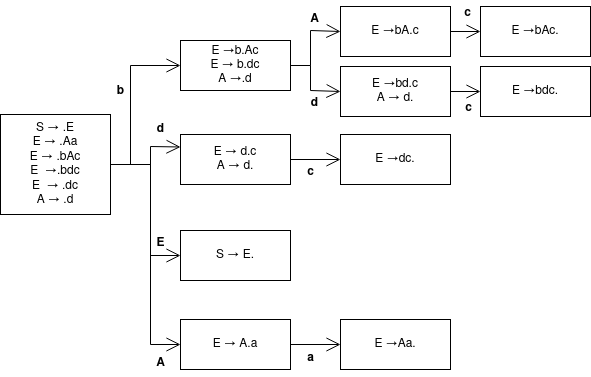
\includegraphics[width=.85\textwidth]{./LR(0).png}
\end{center}
dónde $I_0$ es el estado inicial; $I_1$ es la transición por $E$; $I_2$ es la transición por $A$;
$I_3$ es la transición por $b$; $I_4$ es la transición por $d$. De igual manera, $I_5$ es la transición
desde $I_2$ por $a$; $I_6$ es la transición desde $I_3$ por $A$; $I_7$ es la transición desde
$I_3$ por $d$; $I_8$ es la transición desde $I_4$ por $c$; $I_9$ es la transición desde $I_6$ por
$c$; $I_10$ es la transición desde $I_7$ por $c$.\newline

Luego, análicemos la tabla siguiente y observemos que existen al menos $2$ conflictos \textit{shift/reduce}
y por tanto nuestra gramática no correponde a la clase \textbf{SLR}:

\begin{center}
        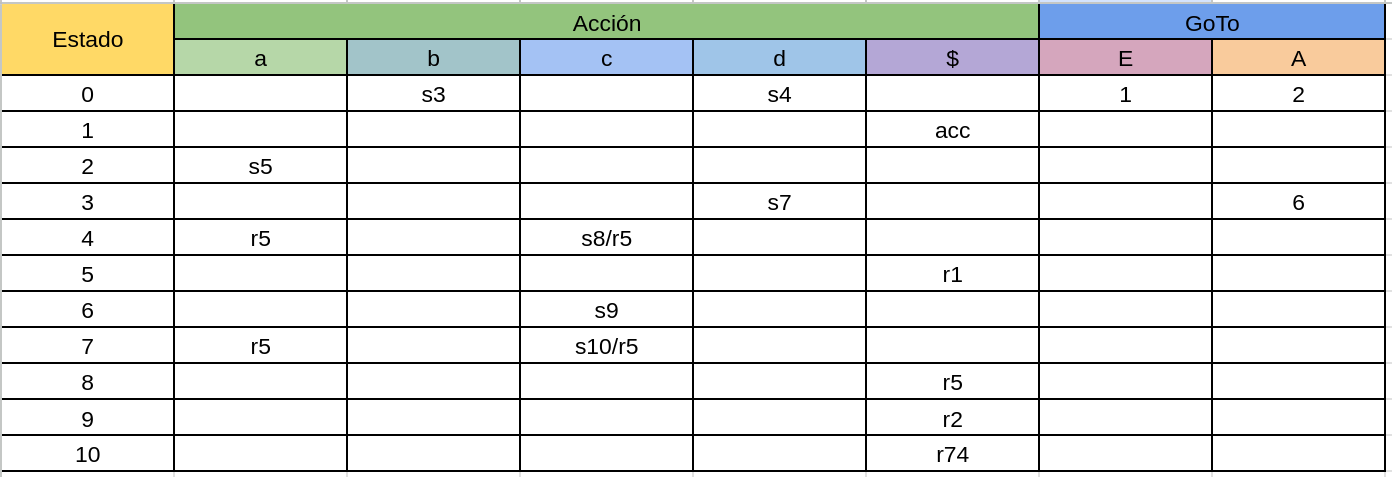
\includegraphics[width=.95\textwidth]{./T.png}
\end{center}

Del análisis \textbf{LR(0)} anterior, encontremos el análisis para \textbf{LR(1)}:\newline

$I_0$:
\begin{eqnarray*}
        S &\rightarrow& .E,   \{a, \$\}\\
        E &\rightarrow& .Aa,  \{a, \$\}\\
        E &\rightarrow& .bAc, \{a, \$\}\\
        E &\rightarrow& .dc,  \{a, \$\}\\
        E &\rightarrow& .bda, \{a, \$\}\\
        A &\rightarrow& .d,   \{a, \$\}
\end{eqnarray*}

$I_1$:
\begin{eqnarray*}
        S &\rightarrow& E., \{\$\}\\
        E &\rightarrow& A.a, \{a\}\\
        E &\rightarrow& .Aa, \{a, \$\}\\
        E &\rightarrow& .bAc, \{a, \$\}\\
        E &\rightarrow& .dc, \{a, \$\}\\
        E &\rightarrow& .bda, \{a, \$\}\\
        A &\rightarrow& .d, \{a, \$\}
\end{eqnarray*}

$I_2$:
\begin{eqnarray*}
    E &\rightarrow&  b.Ac, \{a, \$\}\\
    E &\rightarrow& .bAc, \{a, \$\}\\
    E &\rightarrow& .dc, \{a, \$\}\\
    E &\rightarrow& .bda, \{a, \$\}\\
    A &\rightarrow& .d, \{a, \$\}
\end{eqnarray*}

$I_3$:
\begin{eqnarray*}
    E &\rightarrow& bd.a, \{a, \$\}\\
    E &\rightarrow& .bda, \{a, \$\}\\
    A &\rightarrow& .d, \{a, \$\}
\end{eqnarray*}

$I_4$:
\begin{eqnarray*}
        E &\rightarrow& bda., \{a, \$\}\\
        A &\rightarrow& .d, \{a, \$\}
\end{eqnarray*}

$I_5$:
\begin{eqnarray*}
        E &\rightarrow& .dc, \{a, \$\}\\
        E &\rightarrow& .bda, \{a, \$\}\\
        A &\rightarrow& .d, \{a, \$\}
\end{eqnarray*}

$I_6$:
\begin{eqnarray*}
        E &\rightarrow& d.c, \{a, \$\}\\
        A &\rightarrow& d., \{a, \$\}
\end{eqnarray*}

$I_7$:
\begin{eqnarray*}
        E &\rightarrow& dc., \{a, \$\}\\
        A &\rightarrow& d., \{a, \$\}
\end{eqnarray*}

Minimizando estados tenemos que

$I_1$:
\begin{eqnarray*}
        S &\rightarrow& E., \{\$\}\\
        E &\rightarrow& A.a, \{a\}\\
        E &\rightarrow& .Aa, \{a, \$\}\\
        E &\rightarrow& .bAc, \{a, \$\}\\
        E &\rightarrow& .dc, \{a, \$\}\\
        E &\rightarrow& .bda, \{a, \$\}\\
        A &\rightarrow& .d, \{a, \$\}
\end{eqnarray*}

$I_2$:
\begin{eqnarray*}
    E &\rightarrow&  b.Ac, \{a, \$\}
\end{eqnarray*}

$I_3$:
\begin{eqnarray*}
    E &\rightarrow& bd.a, \{a, \$\}\\
\end{eqnarray*}

$I_4$:
\begin{eqnarray*}
        E &\rightarrow& bda., \{a, \$\}\\
\end{eqnarray*}

$I_5$:
\begin{eqnarray*}
        E &\rightarrow& d.c, \{a, \$\}\\
        A &\rightarrow& d., \{a, \$\}
\end{eqnarray*}

Por lo anteriores pasos, es suficiente para probar que (en efecto)
nuestra gramática pertenece a \textbf{LALR.}\newline

Por último, veamos que la cadena \code{bdc} es producida por la gramática en el parser \textbf{LALR}
como se muestra a continuación:
\begin{eqnarray*}
        S &\rightarrow& E\\
          &\rightarrow& bAc\\
          &\rightarrow& bdc.\\
\end{eqnarray*}
